\documentclass[tikz]{standalone}
\usepackage{pgfplots}
\pgfplotsset{compat=1.15}
\usepackage{mathrsfs}
\usetikzlibrary{arrows,calc}
\usepackage{tkz-euclide}

\pagestyle{empty}

\definecolor{AngleClr}{rgb}{0,0.39215686274509803,0}
\definecolor{ShapeClr}{rgb}{0.6,0.2,0}

\begin{document}

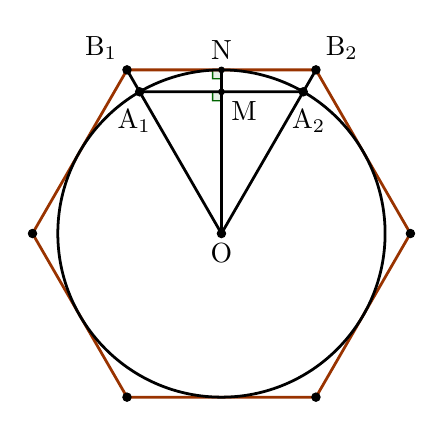
\begin{tikzpicture}[scale=.75]
\tkzSetUpLine[line width=1pt,color=black]
\tkzSetUpPoint[fill=black]

\tkzDefPoints{0/0/P0,3.2/0/P1}

\tkzDefRegPolygon[side,sides=6](P0,P1)

\tkzDefMidPoint(P4,P5) \tkzGetPoint{M}
%\tkzInterLL(N,NN)(M,MM) \tkzGetPoint{O}

\tkzDefCircle[circum](P1,P2,P3) \tkzGetPoint{O}
% \tkzInterLL(O,P5)(P4,P6) \tkzGetPoint{M}

\tkzInterLC(O,P4)(O,M) \tkzGetPoints{b}{B2}
\tkzInterLC(O,P5)(O,M) \tkzGetPoints{B1}{b}
\tkzDefMidPoint(B1,B2) \tkzGetPoint{N}

\tkzFillPolygon[fill=white](P1,P2,P3,P4,P5,P6)

\tkzMarkRightAngles[line width=0.5pt, size=.15,color=AngleClr,fill=AngleClr,fill opacity=0.1](O,M,P5)
\tkzMarkRightAngles[line width=0.5pt, size=.15,color=AngleClr,fill=AngleClr,fill opacity=0.1](O,N,B1)
\tkzDrawPolygon[color=ShapeClr](P1,P2,P3,P4,P5,P6)


\tkzDrawCircle[line width=1pt,black](O,M)
\tkzDrawSegments(O,P4 O,P5 O,M B1,B2)

\tkzDrawPoints[size=3](P1,P2,P3,P4,P5,P6,O,B1,B2)
\tkzDrawPoints[size=2](M,N)

\tkzLabelPoint[below](O){$\rm O$}
\tkzLabelPoint[above](M){$\rm N$}
\tkzLabelPoint[above left](P5){$\rm B_1$}
\tkzLabelPoint[above right](P4){$\rm B_2$}
\tkzLabelPoint[below right](N){$\rm M$}

\tkzLabelPoint[yshift=-0.1cm,xshift=-0.07cm](B1){$\rm A_1$}
\tkzLabelPoint[yshift=-0.1cm,xshift=0.07cm](B2){$\rm A_2$}

\end{tikzpicture}

\end{document}
